\chapter{Erste Übungen mit Java: Turtle-Grafik}
\renewcommand{\chaptertitle}{Erste Übungen mit Java: Turtle-Grafik}

\lehead[]{\sf\hspace*{-2.00cm}\textcolor{white}{\colorbox{lightblue}{\parbox[c][0.70cm][b]{1.60cm}{
\makebox[1.60cm][r]{\thechapter}\\ \makebox[1.60cm][r]{ÜBUNG}}}}\hspace{0.17cm}\textcolor{lightblue}{\chaptertitle}}
\rohead[]{\textcolor{lightblue}{\chaptertitle}\sf\hspace*{0.17cm}\textcolor{white}{\colorbox{lightblue}{\parbox[c][0.70cm][b]{1.60cm}{\thechapter\\
ÜBUNG}}}\hspace{-2.00cm}}
%\chead[]{}
\rehead[]{\textcolor{lightblue}{AvHG, Inf, My}}
\lohead[]{\textcolor{lightblue}{AvHG, Inf, My}}


\section{Turtle-Grafik}

Zum Einstieg in die Programmierung mit der Sprache Java werden wir mit einer
sogenannten Turtle-Grafik geometrische Figuren zeichnen. Bei der Turtle-Grafik
stellt man sich vor, dass ein Roboter (die Schildkröte, engl. „turtle“) einen
Stift auf einer Zeichenfläche hin und her bewegt.

Kopiere dir die Dateien \myFile{Turtle.java} und
\myFile{TurtleGrafik.java} aus dem Kurs-Repository in dein eigenes Repository.

Erzeuge dazu zunächst ein neues \emph{Package} unterhalb des \myFile{src}
Ordners in deinem eigenen Projekt (Rechtsklick auf \myPMI{src} $\rightarrow$
\myPMI{src} $\rightarrow$ \myPMI{Package}). Als Name für das Package bietet
sich \myUserInput{turtle} an. Package-Namen werden üblicherweise komplett aus
kleinbuchstaben gebildet.

Die Datei \myFile{TurtleGrafik.java} enthält bereits ein halb fertiges
Java-Programm mit einer Reihe von Schaltflächen (engl. Buttons). Du musst noch
den Code einfügen, der ausgeführt wird, wenn man auf die Buttons drückt. Nur der
Button \myPMI{Löschen} ist schon fertig programmiert.


\subsection{Kommandos der Turtle}

\subsubsection{Vorwärts oder rückwärts gehen}

\begin{lstlisting}
t.vor(pixel);
\end{lstlisting}

Bewegt die Turtle um die angegebene Anzahl von Pixeln vorwärts. Wenn ein negativer Wert übergeben
wird, geht die Turtle rückwärts.

\subsubsection{Drehen}

\begin{lstlisting}
t.drehen(winkel);
\end{lstlisting}

Dreht die Turtle um den angegebenen Winkel gegen den Uhrzeigersinn. Wenn ein
negativer Wert übergeben wird, dreht sich die Turtle im Uhrzeigersinn.

\begin{minipage}{0.70\textwidth}
Beispiel

\begin{lstlisting}
t.vor(50);       æ// 50 Pixel vorwärts gehen
æt.drehen(-90);   æ// um 90 Grad im Uhrzeigersinn drehen
æt.vor(100);
t.drehen(-90);
t.vor(50);
\end{lstlisting}

Was für eine Figur wird gezeichnet?
\end{minipage}\hfill
\begin{minipage}{0.30\textwidth}
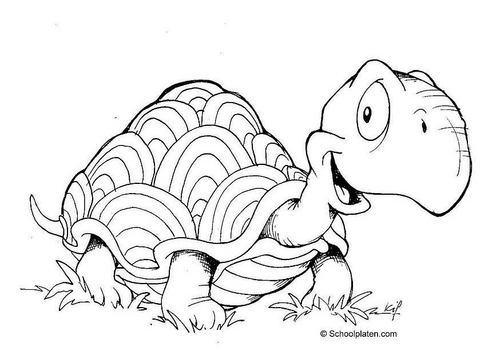
\includegraphics[width=1.0\textwidth]{./inf/SEKII/05_Java_TurtleGrafik/schildkroete.jpg}
% Lizens: http://www.schulbilder.org/malvorlage-schildkroete-i2883.html
% "All images can be used for private educational, non-commercial purposes."
\end{minipage}

\section{Programmieraufgaben zur Turtle-Grafik}

\subsection{Aufgabe 1: Gleichseitiges Dreieck}

Zeichne ein gleichseitiges Dreieck. 

\begin{minipage}{0.80\textwidth}
Überlege dir dazu zunächst, wie groß die Innenwinkel in einem gleichseitigen
Dreieck sein müssen. Die Turtle muss sich allerdings um den Außenwinkel drehen.
Wie groß ist der?
\end{minipage}\hfill
\begin{minipage}{0.1\textwidth}
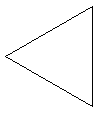
\includegraphics[width=1.0\textwidth]{./inf/SEKII/05_Java_TurtleGrafik/Aufgabe1.png}
\end{minipage}

\subsection{Aufgabe 2: Quadrat}

\begin{minipage}{0.50\textwidth}
\begin{compactenum}[a)]

\item Zeichne ein Quadrat mit einer Seitenlänge von 200 Pixeln.
Programmiere dazu eine kleine while-Schleife, in der du
viermal hintereinander um 200 Pixel vorgehst und die Turtle
anschließend um $90^\circ$ Grad gegen den Uhrzeigersinn drehst.

\item Erweitere das Quadrat so, dass du zusätzlich noch die Diagonalen
einzeichnest. Nach Teil (a) blickt die Turtle wieder nach oben. Wenn du sie
jetzt $45^\circ$ Grad gegen den Uhrzeigersinn drehst, hat sie die richtige
Blickrichtung für die erste Diagonale. Die Länge der Diagonale kannst du mit dem
Satz des Pythagoras berechnen.
\end{compactenum}
\end{minipage}\hfill
\begin{minipage}{0.2\textwidth}

\includegraphics[width=1.0\textwidth]{./inf/SEKII/05_Java_TurtleGrafik/Aufgabe2a.png}
\end{minipage}\hfill
\begin{minipage}{0.2\textwidth}

\includegraphics[width=1.0\textwidth]{./inf/SEKII/05_Java_TurtleGrafik/Aufgabe2b.png}
\end{minipage}


\subsection{Aufgabe 3: Sechseck}

Bewege die Turtle mit einer \myUserInput{while}-Schleife 6-mal hintereinander um
100 Pixel vorwärts und drehe sie dann um $60^\circ$ gegen den Uhrzeigersinn. Es
entsteht ein Sechseck.


\subsection{Aufgabe 4: Achteck}

Bewege die Turtle mit einer \myUserInput{for}-Schleife 8-mal hintereinander um
100 Pixel vorwärts und drehe sie dann um $45^\circ$ gegen den Uhrzeigersinn. Es
entsteht ein Achteck.


\subsection{Aufgabe 5: Treppe}

\begin{compactenum}[a)]

\item Zeichne in einer Schleife die links abgebildete Figur, die aus 15
 Treppenstufen besteht. Die Höhe und Breite jeder einzelnen Stufe beträgt 10
 Pixel.

\item Hänge an die Figur eine zweite Treppe an, die spiegelverkehrt nach unten
 führt.
\end{compactenum}

\hspace{5mm}
\begin{minipage}{0.3\textwidth}
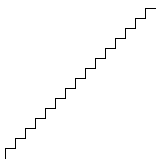
\includegraphics[width=1.0\textwidth]{./inf/SEKII/05_Java_TurtleGrafik/Aufgabe5a.png}
\end{minipage}\hfill
\begin{minipage}{0.6\textwidth}
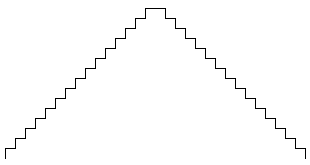
\includegraphics[width=1.0\textwidth]{./inf/SEKII/05_Java_TurtleGrafik/Aufgabe5b.png}
\end{minipage}
 
 
\subsection{Aufgabe 6: Spirale}

Zeichne eine Spirale. Lege dazu eine lokale Variable laenge an und setze sie am
Anfang auf 15. Führe nun in einer Schleife 64 mal hintereinander die folgenden
Schritte aus:

\begin{compactitem}
\item Bewege die Turtle um die laenge nach vorne.
\item Drehe die Turtle um $90^\circ$ Grad gegen den Uhrzeigersinn.
\item Verlängere die Variable laenge um 1/15 ihrer aktuellen Länge.
\end{compactitem}


\subsection{Aufgabe 7: Verschachtelte Quadrate}

\begin{compactenum}[a)]
\item Programmiere eine Methode \verb|quadrat()|, die ein Quadrat einer
beliebigen Länge zeichnen kann. Die Methode erhält die Seitenlänge als
Parameter übergeben. Sie zeichnet in einer Schleife 4-mal hintereinander eine
Linie der angegebenen Länge und dreht sich anschließen um $90^\circ$ im
Uhrzeigersinn.

\item Zeichne in einer Schleife 22 ineinander liegende Quadrate, in dem du
jeweils die Methode \verb|quadrat()| aufrufst. Die Seitenlänge der Quadrate soll
immer erhöht werden. Das erste Quadrat erhält die Seitenlänge 4. Bei jedem
nachfolgenden Quadrat wird die Seitenlänge um $1/4$ ihrer aktuellen Länge
erhöht. Es entsteht eine hübsche Figur.
\end{compactenum}


\subsection{Aufgabe 8: Achtzehn Sechsecke}

\begin{compactenum}[a)]
\item Programmiere eine parameterlose Methode \verb|sechseck()|, die ein
Sechseck mit einer Seitenlänge von 100 Pixeln malt. Du kannst dazu deine Lösung
von Aufgabe 3 wieder verwenden.

\item Rufe in einer Schleife 18-mal hintereinander die Methode \verb|sechseck()|
auf und drehe dich anschließend jeweils um $20^\circ$ gegen den Uhrzeigersinn.
\end{compactenum}


\subsection{Aufgabe 9: Sechseck aus Dreiecken}

\begin{compactenum}[a)]
\item Programmiere eine parameterlose Methode \verb|dreieck()|, die ein Dreieck
mit einer Seitenlänge von 100 Pixeln malt. Du kannst dazu deine Lösung von
Aufgabe 1 wieder verwenden.

\item Rufe in einer Schleife 6-mal hintereinander die Methode \verb|dreieck()|
auf und drehe dich anschließend auf geeignete Weise, so dass die abgebildete
Figur entsteht.
\end{compactenum}

\begin{center}
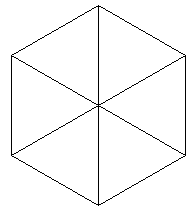
\includegraphics[width=0.2\textwidth]{./inf/SEKII/05_Java_TurtleGrafik/Aufgabe9.png}
\end{center}


\subsection{Aufgabe 10: Figur aus vier Dreiecken}

Rufe in einer Schleife 4-mal hintereinander die Methode \verb|dreieck()| auf und
drehe dich anschließend auf geeignete Weise, so dass die abgebildete Figur entsteht. 

Beachte, dass du die Turtle vor dem Beginn der Schleife in eine geeignete
Ausgangsposition drehen musst.

\begin{center}
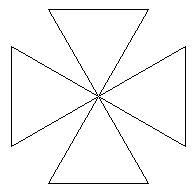
\includegraphics[width=0.2\textwidth]{./inf/SEKII/05_Java_TurtleGrafik/Aufgabe10.png}
\end{center}


\subsection{Aufgabe 11: Stern aus Dreiecken}

Zeichne den abgebildeten Stern, in dem du in einer Schleife die Methode
\verb|dreieck()| 6-mal hintereinander aufrufst und dich anschließend geeignet
drehst.

\begin{center}
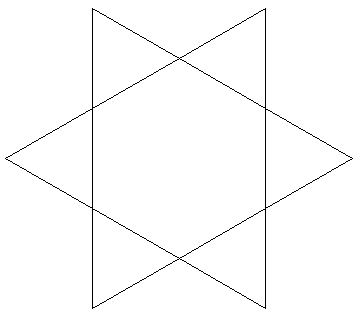
\includegraphics[width=0.2\textwidth]{./inf/SEKII/05_Java_TurtleGrafik/Aufgabe11.png}
\end{center}
